\documentclass[10pt,a4paper]{report}


\usepackage{amsmath}
\usepackage[utf8]{inputenc}
\usepackage{amsmath}
\usepackage{amsfonts}
\usepackage{amssymb}
\usepackage{calrsfs}
\usepackage[left=2cm,right=2cm,top=2cm,bottom=2cm]{geometry}
\usepackage[mathscr]{euscript}

%%%for drawing commutative diagrams.%%%%%%
\usepackage{tikz-cd}  
%%%%%%%%%%%%%%%%%%%%%%%%%%%%%%%%%%%%%%%%%%

%%%%%%%%%%for changing margin
\def\changemargin#1#2{\list{}{\rightmargin#2\leftmargin#1}\item[]}
\let\endchangemargin=\endlist 

\newenvironment{proof}
{\begin{changemargin}{1cm}{0.5cm} 
	}%your text here
	{\end{changemargin}
}
%%%%%%%%%%%%%%%%%%%%%%%%%%%%%

\begin{document}
\newcommand{\thm}{\textbf{Theorem) }}
\newcommand{\thmnum}[1]{\textbf{Theorem #1) }}
\newcommand{\defi}{\textbf{Definition) }}
\newcommand{\definum}[1]{\textbf{Definition #1) }}
\newcommand{\lem}{\textbf{Lemma) }}
\newcommand{\lemnum}[1]{\textbf{Lemma #1) }}
\newcommand{\prop}{\textbf{Proposition)}}
\newcommand{\propnum}[1]{\textbf{Proposition #1) }}
\newcommand{\corr}{\textbf{Corollary) }}
\newcommand{\corrnum}[1]{\textbf{Corollary #1) }}
\newcommand{\pf}{\textbf{proof) }}


\newcommand{\lap}{\triangle} %%Laplacian
\newcommand{\s}{\vspace{10pt}}
\newcommand{\bull}{$\bullet$}
\newcommand{\sta}{$\star$}
\newcommand{\reals}{\mathbb{R}}

\newcommand{\eop}{\hfill  \textsl{(End of proof)} $\square$} %end of proof
\newcommand{\eos}{\hfill  \textsl{(End of statement)} $\square$} %end of proof


\newcommand{\intN}{\mathbb{Z}_N}
\newcommand{\nat}{\mathbb{N}}
\newcommand{\norms}[2]{\parallel #1 \parallel_{#2}}
\newcommand{\avg}{\mathbb{E}}
\newcommand{\prob}{\mathbb{P}}
\newcommand{\borel}{\mathscr{B}}
\newcommand{\EE}{\mathscr{E}}
\newcommand{\cov}{\text{Cov}}
\newcommand{\var}{\text{Var}}

\newcommand{\newday}{===============================================================}

\setlength\parindent{0pt}

\chapter*{Advanced Probability}
\s

\begin{large}
-Martingales
\end{large}

\newday

(15th October 2018, Monday)
\s

\section*{Chapter 2. Martingales in Discrete Time}

\subsection*{2.1. Definitions.}

\newcommand{\F}{\mathscr{F}}
\newcommand{\G}{\mathscr{G}}

Let $(\Omega, \F, \prob)$ be a probability space.


\begin{itemize}
\item A \textbf{Filtration} for $(\Omega, \F, \prob)$ is a sequence $(\F_n)_{n\geq 0}$ of $\sigma$-algebras s.t. for all $n \geq 0$, we have
\begin{align*}
\F_n\subset \F_{n+1} \subset \F
\end{align*}
Set $F_{\infty} = \sigma(\F_n:n\geq 0)$ then $\F_{\infty} \subset \F$. We allow $\F_{\infty} \neq \F$. We interpret $n$ as times and $\F_n$ as the extent of knowledge at time $n$.

\item A \textbf{Random process(in discrete time)} is a sequence of random variables $(X_n)_{n\geq 0}$. It has a natural filtration $(F_n^X)_{n\geq 0}$ given by
\begin{align*}
\F_n^X = \sigma(X_0, \cdots, X_n)
\end{align*}
That is, the knowledge obtained from $X_n$ by time $n$. We say $(X_n)_{n\geq 0}$ is \textbf{adapted to} $(\F_n)_{n\geq 0}$ if $X_n$ is $\F_n$-measurable for all $n\geq 0$. This is equivalent to having $\F_n^X \subset \F_n$, for all $n \geq 0$. (Here, $X_n$ are real-valued) 

\item We would say $(X_n)_{n\geq 0}$ is \textbf{integrable} if $X_n$ is integrable for all $n\geq 0$.

\item A \textbf{martingale} is an \emph{adapted, integrable random process} $(X_n)_{n\geq 0}$ s.t. for all $n\geq 0$,
\begin{align*}
\avg[X_{n+1} |\F_n] = X_n \quad \text{a.s.}
\end{align*}
In the case $\avg[X_{n+1} |\F_n] \leq X_n$ a.s., $(X_n)_n$ is called a \textbf{super-martingale} and in the case $\avg[X_{n+1} |\F_n] \geq X_n $ a.s., $(X_n)_n$ is called a \textbf{sub-martingale}.
\end{itemize}

\newcommand{\randp}{(X_n)_{n \geq 0}} %a random process

\subsection*{Optional Stopping}

\begin{itemize}
\item A random variable $T:\Omega \rightarrow \{ 0,1,2,\cdots \} \cup \{\infty\}$ is a \textbf{stopping time} if $\{ T\leq n\}\in \F_n$ for all $n \geq 0$.

\item For a stopping time $T$, we set $\F_T = \{ A\in \F_{\infty} : A\cap \{ T\leq n \} \in \F_n$ for all $n\geq 0 \}$. It is easy to check $\F_T$ is indeed a $\sigma$-algebra and that if $T(\omega) = n$ for all $\omega \in \Omega$, then $T$ is a stopping time and $\F_T = \F_n$.

\item Given $X$, define $X_T(\omega) = X_{T(\omega)}(\omega)$ whenever $T(\omega) <\infty$ and define the \textbf{stopped process} $X^T$ by
\begin{align*}
X_n^T (\omega)  = X_{T(\omega) \wedge n} (\omega) \quad \text{for } n\geq 0
\end{align*}
\end{itemize}

\propnum{2.2.1.} Let $X$ be an adapted process. Let $S$, $T$ be stopping times for $X$. Then
\begin{itemize}
\item[(a)] $S\wedge T$ is a stopping time for $X$.
\item[(b)] $\F_T$ is a $\sigma$-algebra.
\item[(c)] If $S\leq T$ then $\F_S \subset \F_T$.
\item[(d)] $X_T 1_{T<\infty}$ is an $\F_T$-measurable random variable.
\item[(e)] $X^T$ is adapted.
\item[(f)] If $X$ is integrable, then $X^T$ is also integrable.
\end{itemize}

\begin{proof}
\pf
\begin{itemize}
\item[(a)] $\{ S \wedge T \leq n \} = \{S  \leq n \} \cup \{ T \leq n\} \in \F_n$ for all $n\geq 0$, so $S\wedge T$ is a stopping times

\item[(b)] Directly from the definition, we see that $\phi \F_T$. Also, given $A\in \ \F_T$ and a sequence $(A_m)_m \subset \F_T$, we have
\begin{align*}
& A^c \cap \{T\leq n \} = \{T\leq n\} - A \cap \{T\leq n \} \in \F_n \quad \Rightarrow  A^c \in \F_T \\
&(\cup_m A_m) \cap \{T\leq n\} =  \cup_m (A_m \cap \{T\leq n\}) \in \F_n \quad \Rightarrow \cup_m A_m \in \F_T
\end{align*}
hence $\F_T$ is a $\sigma$-algebra.

\item[(c)] Let $A\in \F_S$. Then $A\cap \{T\leq n\} = A \cap \{S\leq n\} \cap \{T \leq n\} \in \F_n$, hence $A \in \F_T$.

\item[(d)] For each $t\in \reals$, we have $\{X_T 1_T >t \} = \cup_m \{X_m >t, T=n \}$ so for any $n\geq 0$,
\begin{align*}
\{X_T 1_T >t \} \cap \{T\leq n\} = \cup_{m=1}^n \{X_m >t, T=n \} \in \F_n
\end{align*}
and so $X_T 1_T$ is $\F_T$-measurable.

\item[(e)] By definition of being a stopping time, for any $t\in \reals$, 
\begin{align*}
\{(X^T)_n >t\} = \{T>n, X_n>t\} \cup \Big( \cup_{m=0}^n \{T=m, X_m>t \} \Big)\in \F_n
\end{align*}
so $X^T$ is adapted.

\item[(f)] First consider the case where $X$ is non-negative integrable. Then
\begin{align*}
\avg(X^T_n) = \avg(\avg(X_n^T |T)) = \sum_{m\geq n} \prob(T=m) \avg(X_m) + \prob(T>n) \avg(X_n) < \infty
\end{align*}
for any $n$, so we have the result for non-negative $X$.

\quad For the general case, divide $X$ into a non-negative and a negative part.
\end{itemize}
\eop
\end{proof}
\s

\thmnum{2.2.2} \emph{(Optional stopping theorem)} Let $X$ be a super-martingale and let $S,T$ be \emph{bounded} stopping times with $S \leq T$ a.s. Then
\begin{align*}
\avg[X_T] \leq \avg[X_S]
\end{align*}
\begin{proof}
\pf Fix $n\geq 0$ such that $T\leq n$ a.s. Then
\begin{align*}
X_T &= X_S + \sum_{S\leq k <T} X_{k+1} - X_k  \\
&= X_S + \sum_{k=0}^n (X_{k+1} - X_k) 1_{S\leq k <T}
\end{align*}
Now $\{S\leq k\}$ is in $\F_k$ and $\{T>k\}$ is in $\F_k$, so
\begin{align*}
\avg[(X_{k+1} - X_k)1_{S\leq k <T}  ] &= \avg [\avg[ (X_{k+1} - X_k) 1_{S\leq k<T} |\F_k ]] \\
& = \avg[ \avg [  X_{k+1} -X_k | \F_k ] 1_{S\leq k < T} ]
\end{align*}
but since $(X_n)$ was a super-martingale,  $\avg [  X_{k+1} -X_k | \F_k ] \leq 0$ a.s. and therefore $\avg[(X_{k+1} - X_k)1_{S\leq k <T}  ] \leq 0$ a.s. Hence $\avg(X_T) \leq \avg(X_S)$.

\eop
\end{proof}
\s

\bull Note that $X$ is a sub-martingale \emph{if and only if} ($-X$) is a super-martingale, and that $X$ is a martingale \emph{if and only if} $X$ and ($-X$) are super-martingales. Hence, we obtain sub-martingale and martingale versions of the theorem :
\begin{align*}
&\text{If } (X_n) \text{ is a sub-martingale, } \avg[X_T] \geq \avg[X_S] \\
&\text{If } (X_n) \text{ is a martingale, } \avg[X_T] = \avg[X_S]
\end{align*}
\s

\thmnum{2.2.3.} Let $X$ be an adapted integrable process. Then the followings are equivalent.
\begin{itemize}
\item[(a)] $X$ is a super-martingale. 
\item[(b)] for all bounded stopping times $T$ and stopping time $S$,
\begin{align*}
\avg(X_T |\F_S) \leq X_{S\wedge T} \quad \text{a.s.},
\end{align*}
\item[(c)] for all stopping times $T$, $X_T$ is a super-martingale,
\item[(d)] for all bounded stopping times $T$ and all stopping times $S$ with $S\leq T$ a.s,
\begin{align*}
\avg(X_T) \leq \avg(X_S)
\end{align*}
\end{itemize}

$\star$ The theorem gives an inverse statement of the optional stopping theorem.
\s

\begin{proof}
\pf

\begin{itemize}
\item[(a) $\Rightarrow$ (b)] Suppose $X$ is a super-martingale and $S,T$ are stopping times. Let $T\leq n$, for some $n<\infty$. Then
\begin{align*}
X_T = X_{S\wedge T} + \sum_{k=0}^T (X_{k+1} - X_k) 1_{S\leq k<T} \cdots \cdots (*)
\end{align*}
Let $A \in \F_S$. Then $A\cap \{ S\leq k\}\in \F_k$ and $\{T>k\} \in \F_k$ so
\begin{align*}
\avg[(X_{k+1} - X_k) 1_{S\leq k<T} 1_A] =\avg[\avg[(X_{k+1} - X_k) 1_{S\leq k<T} 1_A|\F_k]] \leq 0
\end{align*}
and
\begin{align*}
\avg[(X_T - X_{S\wedge T}) 1_A] = & \avg[\sum_{n=0}^T (X_{k+1} - X_k) 1_{S\leq k<T} 1_A] \leq 0 \\
& \Rightarrow \quad \avg[ X_T 1_A] \leq \avg[X_{S\wedge T} 1_A] \\
\end{align*}
But since this inequality is true for any $A\in \F_S$ and noting that $X_{S\wedge T} \in \F_S)$, we see
\begin{align*}
\avg[X_T |\F_S] \leq X_{S\wedge T} \quad \text{a.s.}
\end{align*}
\s

The inclusions (b)$\Rightarrow$(c) and (c)$\Rightarrow$(d) are obvious.
\s

\item[(d) $\Rightarrow$ (a)] Let $m\leq n$ and $A\in \F_n$. Set $T= m1_A + n1_{A^c}$. Then $T$ is a stopping with $T\leq n$. Then
\begin{align*}
\avg(X_n 1_A -X_m 1_A) = \avg(X_n) - \avg(X_T) \leq 0
\end{align*}
(note, if $\omega \in A$ then $(X_n1_A - X_m1_A)(\omega) = X_n(\omega) -X_m(\omega)$ and $0$ otherwise) so
\begin{align*}
\avg[X_n | \F_m] \leq X_m
\end{align*}
\end{itemize}
\eop
\end{proof}
\s

\newday

(17th October, Wednesday)
\s

\subsection*{2.3. Doob's upcrossing inequality}

\begin{itemize}
\item Let $X$ be a random process and let $a,b\in \reals$ s.t. $a<b$. Fix $\omega \in \Omega$. By an \textbf{upcrossing} of $[a,b]$ by $X(\omega)$, we mean an interval of times $\{j,j+1, \cdots, k\}$ s.t. $X_j(\omega) <a$, $X_k(\omega) >b$.

\item Write $U_n[a,b](\omega)$ for the number of disjoint upcrossings contained in $\{0,1,\cdots,n\}$, and $U_n[a,b] \nearrow U[a,b]$ as $n\rightarrow \infty$.
\end{itemize}
\s

\begin{center}
	\begin{figure}
		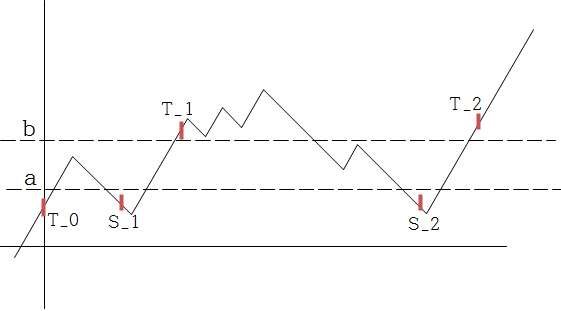
\includegraphics[scale=0.5]{upcrossing}
	\end{figure}
\end{center}

\thmnum{2.3.1.}(Doob's upcrossing inequality) Let $X$ be a \emph{super-martingale}. Then
\begin{align*}
(b-a) \avg[U[a,b]] \leq \sup_{n\geq 0} \avg[(X_n-a)^{-}]
\end{align*}
(Recall, $x^- = (-x) \vee 0$)
\begin{proof}
Set $T_0 =0$ and define recursively for $k\geq 0$,
\begin{align*}
S_{k+1} = \inf \{m\geq T_k : X_m <a \}, \quad T_{k+1} = \sup \{m\geq S_{k+1} : X_m >b \}
\end{align*}
Note that if $T_k < \infty$, then $\{S_k, S_{k}+1, T_k \}$ is an upcrossing of $[a,b]$ by $X$, and $T_k$ is the time of completion of the $k-th$ upcrossing.
\quad Also note that $U_n [a,b] \leq n$. For $m\leq n$, we have
\begin{align*}
\{U_n[a,b] =m \} = \{T_m \leq n < T_{m+1} \}
\end{align*}
On this event,
\begin{align*}
X_{T_k \wedge n}  - X_{S_k \wedge n} = \begin{cases}
X_{T_k} - X_{S_k} \geq b-a \quad \text{if } k\leq m \\
X_n - X_{S_k} \geq X_n -a \quad \text{if } k =m1, S_{m+1} \leq n \\
0 \quad \text{otherwise}
\end{cases}
\end{align*}
Hence
\begin{align*}
\sum_{k=1}^n (X_{T_k \wedge n} - X_{S_k \wedge n}) &\geq (b-a) U_n[a,b] + X_n - a \\
&\geq (b-a)U_n[a,b] -(X_n -a)^-
\end{align*}
Since $X$ is a super-martingale and $T_k \wedge n$ and $S_k \wedge n$ are \emph{bounded stopping times} with $S_k \leq T_k$, by optional stopping theorem, we have
\begin{align*}
\avg (X_{T_k \wedge n})\leq \avg(X_{S_k \wedge n})
\end{align*}
By $\avg(\sum_{k=1}^n (X_{T_k \wedge n} - X_{S_k \wedge n}))$ we get
\begin{align*}
(b-a) \avg(U_n[a,b]) \leq \sum_{n\geq 0} \avg[(X_n-a)^-]
\end{align*}
Apply monotone convergence, with $n\rightarrow \infty$, then we are done.

\eop
\end{proof}
\s

This theorem does not seem to have any significance at the moment, but it will turn out to be important later on.

\subsection*{2.4. Doob's maximal inequalities.}

\quad Define $X_n^ = \sum_{k\geq n} |X_k|$
\s

In the next two theorems, we see that the martingale(or sub-martingale) property allows us to obtain estimates on this $X_n^*$ in terms of expectations for $X_n$.\\
\s

\thmnum{2.4.1} (Doob's maximal inequality) Let $X$ be a \emph{martingale or a non-negative sub-martingale}. Then for all $\lambda \geq 0$,
\begin{align*}
\lambda \prob(X_n^* \geq \lambda) \leq \avg(|X_n|   1_{\{ X_n^*\geq \lambda \}}) \leq \avg(|X_n|)
\end{align*}
\begin{proof}
\pf If $X$ is a martingale, then $|X|$ is a non-negative sub-martingale. It suffices to consider the case where $X$ is a non-negative sub-martingale.

\quad Set $T = \inf \{ k \geq 0 : X_k \geq \lambda \} \wedge n$. Then $T$ is a stopping time and $T\leq n$, so by optional stopping, has
\begin{align*}
\avg(X_n) \geq \avg(X_T) &= \avg(X_T 1_{X^*_n \geq \lambda}) + \avg(X_T 1_{X^*_n < \lambda}) \\
& = \avg( \lambda 1_{X^*_n \geq \lambda})  + \avg(X_n 1_{X_n^* < \lambda})
\end{align*}
and
\begin{align*}
\avg(X_n 1_{X^* \geq \lambda}) \geq \lambda \prob(X^*_n \geq \lambda)
\end{align*}

\eop
\end{proof}
\s

\thmnum{2.4.2} (Doob's $L^p$-inequality) Let $X$ be a \emph{martingale or a non-negative sub-martingale}. Then, for all $p>1$ and $q = p/(p-1)$, we have
\begin{align*}
\norms{X^*_n}{p} \leq q \norms{X_n}{q} 
\end{align*}
\begin{proof}
\pf Again, it suffices to consider when $X$ is a non-negative sub-martingale. Fix $k < \infty$. Then
\begin{align*}
\avg [ (X^*_n \wedge k)^p  ] &= \avg \int_0^k p \lambda^{p-1} 1_{\{x^*_n \lambda \}} d\lambda \quad \text{(integration by parts)}\\
& = \int_0^k p \lambda^{p-1} \prob(X^*_n \geq \lambda) d\lambda \quad \text{(Fubini)} \\
& \leq \int+0^k p\lambda^{p-2} \avg (X_n 1_{X^*_n \geq \lambda}) d\lambda \quad \text{(Doob's maximal inequaltiy)} \\
& =\frac{p}{p-1} \avg(X_n (X^*_n \wedge k)^{p-1} ) \\
& \leq q \norms{X_n}{p} \norms{X^*_n \wedge k}{p}^{p-1} \quad \text{(H\"{o}lder's inequality)}
\end{align*}
Hence , $\norms{X^*_n \wedge k}{p} \leq q\norms{X_n}{p}$. Apply monotone convergence theorem with $k\rightarrow \infty$, then we have the desired result.

\eop
\end{proof}
\s

Doob's maximal and $L^p$ inequalities have different versions which apply under the same hypothesis to
\begin{align*}
X^* = \sum_{n\geq 0} |X_n|
\end{align*}
since $X^*_n \nearrow X^*$. Letting $n\rightarrow \infty$ in Doob's maximal inequality gives
\begin{align*}
\lambda \prob(X^* \geq \lambda) \lim_{n\rightarrow \infty} \lambda \prob(X^*_n \geq \lambda) \leq \sup_{n\geq 0} \avg(|X_n|)
\end{align*}
We can then replace $\lambda \prob(X^* >\lambda)$ by $\lambda \prob (X^* \geq \lambda)$ by taking limits from the right in $\lambda$.

\quad Similarly, for $p\in (1,\infty)$ by monotone convergence,
\begin{align*}
\norms{X^*}{p} \leq q \sup_{n\geq 0} \norms{X_n}{p}
\end{align*}

\end{document}